\documentclass[11pt]{article}

\usepackage[a4paper,margin=2.4cm]{geometry}
\usepackage{amsmath,amssymb}
\usepackage{booktabs}
\usepackage{siunitx}
\usepackage{graphicx}
\usepackage{xcolor}
\usepackage[hidelinks]{hyperref}
\usepackage{enumitem}

\newcommand{\bplus}{\beta^{+}}
\newcommand{\Cl}[1]{{}^{#1}\mathrm{C}}
\newcommand{\Ox}[1]{{}^{#1}\mathrm{O}}
\newcommand{\Nt}[1]{{}^{#1}\mathrm{N}}
\newcommand{\Rd}{R_{\mathrm d}}
\newcommand{\Rp}{R_{\mathrm p}}
\newcommand{\tirr}{t_{\mathrm{irr}}}
\newcommand{\tdel}{t_{\mathrm{del}}}
\newcommand{\tmeas}{t_{\mathrm{meas}}}
\newcommand{\file}[1]{\texttt{#1}}

\title{The \texttt{ptcryspg4} user guide:\\
running the pipeline and using the scenario}
\author{J.J. G\'omez-Cadenas\\\texttt{jjgomezcadenas@gmail.com}}
\date{Documentation last rebuild: \today}

\begin{document}
\maketitle

\begin{abstract}
\texttt{ptcryspg4} simulates a proton beam stopping in a phantom, records where
positron emitters are created and where their positrons annihilate, and turns that
production into the number of decays a PET scanner would measure. The output is a
detector-independent annihilation source, frozen as a named \emph{scenario} that a
downstream PET simulation reads. This guide is operational: it describes how the
pipeline is organised and run, the phantoms and beams available, how the source is
normalised and how the measured decays are computed, and the format and use of the
scenario data product. The physics behind the source --- induced activity, decay
kinetics, and SOBP field design --- is in the companion physics note
(\file{ptcrysp\_physics.tex}).
\end{abstract}

\section{The pipeline}
\label{sec:pipeline}

The work splits into two parts, joined by CSV files. The first is a Geant4
simulation of a proton beam stopping in a phantom, which records the trail of
positron emitters it leaves along the way. Two ingredients define the run:
\begin{itemize}[nosep]
\item \textbf{A beam} --- protons, either a simple pencil or the more realistic
spread-out Bragg peak (SOBP).
\item \textbf{A phantom} --- a body of material standing in for the region being
treated. \texttt{ptcryspg4} implements five: a homogeneous brain-tissue cylinder,
a homogeneous head, a MIRD head built from three materials (scalp, skull and
brain), the MIRD head with a posterior-fossa tumour (HeadEP), and HeadEP's
homogeneous control (Sec.~\ref{sec:phantom}).
\end{itemize}

The run produces the spatial source; a second, analytic step folds in the
radioactive half-lives and the scanner's acquisition timing to turn the emitters
that were \emph{produced} into the number of decays actually \emph{measured}. This
second step is the handoff.

\begin{center}
\fbox{\parbox{0.95\textwidth}{\ttfamily\small
\textbf{proton run (Geant4)} \hfill \textit{runs once}\\
\hspace*{1em}protons $\to$ phantom $\to$ $\bplus$ emitter produced $\to$ positron annihilates\\
\hspace*{1em}$\Rightarrow$ emitters.csv (production + annihilation points) + run\_meta.csv\\[2pt]
\textbf{handoff (Python)}\\
\hspace*{1em}produced emitters $\to$ decay + acquisition window $\to$ measured count\\
\hspace*{1em}$\Rightarrow$ sampling\_budget\_<scenario>.csv (decays per isotope)\\[2pt]
\hspace*{1em}frozen as a named scenario; a detector simulation reads it
}}
\end{center}

The proton run is expensive and runs \emph{once}; the handoff is cheap and is
repeated for each acquisition timing. The two are described in
Secs.~\ref{sec:transport} and \ref{sec:handoff}, the scenario data product in
Sec.~\ref{sec:scenario}, and the commands in Sec.~\ref{sec:using}.

\section{The proton run}
\label{sec:transport}

\subsection{The beam}
\label{sec:beam}
The standard beam is a spread-out Bragg peak: several proton energies combined so
the dose is flat across the whole target volume. A single mono-energetic pencil is
also available, for simpler tests. The SOBP energy layers and their weights are
designed analytically (the method is in \file{ptcrysp\_physics.tex}); the
operational design and verification are in Sec.~\ref{sec:field}.

\subsection{The phantoms}
\label{sec:phantom}
The five phantoms share the same beam axis ($z$) and the same target-box dose
normalisation; they differ in shape and in how many materials they contain.

\paragraph{Cylinder.} A single homogeneous cylinder with its axis along the beam.
The standard material is brain tissue (\file{G4\_BRAIN\_ICRP}) in a cylinder
\SI{16}{cm} across and \SI{16}{cm} long, a simple stand-in for a head chosen so the
isotope yields can be checked against the published numbers of Parodi
\emph{et al.}\ (2008)~\cite{parodi2008comparison}. The material is selectable: soft
tissue, PMMA (carbon-rich), and water (an almost pure-$\Ox{15}$ source) are also
available. The carbon and oxygen content sets the mix of isotopes; the
$\Ox{15}/\Cl{11}$ ratio is computed directly from the simulation.

\paragraph{Uniform head.} A head-shaped ellipsoid (about \SI{17}{cm} and
\SI{20}{cm} across, \SI{14}{cm} along the beam) filled with a single material,
brain tissue by default. It keeps the homogeneous character of the cylinder but
adds the realistic outer shape, so the beam traverses a varying thickness of
material across its cross-section.

\paragraph{MIRD head.} A layered, anatomically realistic head built from three
nested ellipsoids: a soft-tissue scalp (\file{G4\_TISSUE\_SOFT\_ICRP}), a
cortical-bone skull (\file{G4\_BONE\_CORTICAL\_ICRP}), and a brain-tissue core
(\file{G4\_BRAIN\_ICRP}). The dense bone layer shifts the proton range, so the
SOBP field is designed through the actual scalp/skull/brain path in
water-equivalent depth to land the dose plateau on the target.

\paragraph{HeadEP.} The MIRD head with a tumour: a soft-tissue ellipsoid of
semi-axes $18\times20\times\SI{18}{mm}$ at the posterior-fossa site of a
reference ependymoma --- midline, posterior, inferior (the 4th-ventricle
region), fully inside the brain. The head is turned so its
anterior--posterior axis lies along the beam and the tumour centre sits on
the beam axis: the beam enters through the occiput and travels anterior,
straight at the tumour. The dose target is the tumour itself
(\SI{40}{mm} diameter $\times$ \SI{40}{mm}, at \SI{57}{}--\SI{97}{mm} depth
from the occiput entrance), and the SOBP field is WEPL-designed through the
posterior scalp/skull/brain path. In \file{phantom\_regions.csv} the tumour
is a fourth region that carves the brain.

\paragraph{Uniform HeadEP.} The homogeneity control for HeadEP: the same
envelope, posterior placement, and target window, but brain throughout ---
no scalp/skull layers and no tumour region. Comparing the range-recovery
spread $\sigma_R$ between \file{headep} and \file{uniform\_headep} isolates
what the tissue layering does to the distal edge, with the orientation,
target, and outer attenuation shell held identical.

\paragraph{Construction.} The heads are nested, axis-aligned ellipsoids taken
from the Geant4 MIRD adult-head model with the face and neck dropped: scalp
semi-axes $72\times102\times\SI{87}{mm}$, skull outer surface
$68\times98\times\SI{83}{mm}$, and brain $60\times90\times\SI{65}{mm}$, the
brain centre shifted \SI{10}{mm} toward the crown. The skull is the shell
between its outer ellipsoid and the brain-sized cavity. For the lateral cases
(\file{uniform\_head}, \file{mird\_head}) the head is rotated so the beam
crosses it ear to ear; for HeadEP it is rotated about the transverse axis and
translated so the tumour centre lies on the beam axis, the beam entering
through the occiput. In Geant4 the skull shell is a subtraction solid; in the
data model the same geometry is carried by \file{phantom\_regions.csv} as plain
ellipsoids with a priority each, and one rule serves every consumer --- the
WEPL ray-trace, the validation gates, and the plots: the lowest-priority
region containing a point supplies its material, so the brain carves the skull
shell and the tumour carves the brain with no boolean solids in the data.

\subsection{The physics list}
\label{sec:physics}
The physics list is \file{QGSP\_BIC\_HP}, a hadronic list suited to proton-induced
isotope production, with electromagnetic physics and radioactive decay switched
on\footnote{Geant4's isotope-production cross sections are less finely tuned than
those of FLUKA or dedicated data-driven models, so the absolute yields carry some
bias. The same bias applies to every detector, so it cancels in a ranking; the
source files can be regenerated from a better production map.}.

\subsection{How an emitter is recorded}
\label{sec:production}
As a proton slows down it occasionally undergoes a nuclear reaction with a carbon
or oxygen nucleus, for example $\Ox{16}(p,pn)\Ox{15}$ or $\Cl{12}(p,pn)\Cl{11}$.
The leftover nucleus, created essentially at rest, is sometimes one of the positron
emitters in Table~\ref{tab:iso}. It later decays, the positron is transported over
its short range, and it annihilates. For each emitter, two points are recorded:
\begin{itemize}[nosep]
\item the \textbf{production point} --- where the emitter was made (the truth map
of where the beam created activity);
\item the \textbf{annihilation point} --- where the two \SI{511}{keV} photons are
born (the source a detector would see).
\end{itemize}
The distance between the two is the positron range for that event, so the file
already carries the resolution floor that the positron range imposes.

An emitter stays put between production and decay, so its annihilation point is
fixed by geometry alone, and its timing is supplied later by the handoff
(Sec.~\ref{sec:handoff}). The prompt de-excitation $\gamma$ of $\Cl{10}$ and
$\Ox{14}$, and secondary neutrons, are not tracked.

\paragraph{How the run records it.} An emitter is identified by the nucleus
itself: any new track whose $(Z,A)$ matches one of the five isotopes of
Table~\ref{tab:iso} is tagged, whatever reaction made it. Geant4 decays the
tagged nucleus through its standard radioactive-decay process, within the same
event; the positron whose parent is a tagged nucleus supplies both points ---
its vertex is the production point, and where its track ends is the
annihilation point. Geant4 samples the true $\bplus$/EC branching, so the
recorded emitters are the produced nuclei times the $\bplus$ branching ratio
($\gtrsim\SI{99}{\percent}$ for these species): one row per $\bplus$ decay. A
positron that crosses from the phantom into the surrounding air is stopped at
the surface, which pins its annihilation point to the boundary --- the
$\sim$\SI{0.6}{\percent} pinned fraction quoted in Sec.~\ref{sec:files}. Its
\SI{511}{keV} photons are not generated here; the downstream simulation emits
the pair from the recorded point.

\begin{table}[h]
\centering
\caption{The positron emitters, with half-lives and the energy that governs the
positron range. A \SI{100}{\percent} $\bplus$ branch is assumed in the handoff.}
\label{tab:iso}
\begin{tabular}{lccl}
\toprule
Isotope & $T_{1/2}$ & $\bplus$ endpoint (MeV) & Main production channel \\
\midrule
$\Ox{15}$ & \SI{122}{s}   & 1.74 & $\Ox{16}(p,pn)\Ox{15}$ \\
$\Cl{11}$ & \SI{1223}{s}  & 0.96 & $\Cl{12}(p,pn)\Cl{11}$ \\
$\Nt{13}$ & \SI{598}{s}   & 1.19 & on O / N \\
$\Cl{10}$ & \SI{19.3}{s}  & 1.91 & prompt $\gamma$ \SI{718}{keV} \\
$\Ox{14}$ & \SI{70.6}{s}  & 1.81 & prompt $\gamma$ \\
\bottomrule
\end{tabular}
\end{table}

\subsection{Setting the absolute scale}
\label{sec:scale}
The number of simulated protons is arbitrary, so on its own the emitter count has
no absolute meaning. To fix the scale, the dose deposited in a target box inside
the phantom is also scored. The ratio of the two --- emitters per unit dose ---
gives the production for a clinical dose. The standard scale is \SI{1}{Gy} in the
target: from the simulated dose, the number of protons needed to deliver it
($N_p(\SI{1}{Gy})=\file{n\_protons}/\file{target\_dose\_Gy}$) is computed, and the
production is scaled accordingly. This provides the $P_j$ that the decay kinetics
consume (\file{ptcrysp\_physics.tex}, Eq.~3).

Two tallies implement the scoring. The whole-phantom dose
(\file{dose\_total\_Gy}) comes from a Geant4 scorer attached to the phantom
volumes. The target box is a scoring region rather than a geometry volume --- a
cylinder of the target's radius and depth span whose mass follows analytically
from the material at its centre --- and every energy-depositing step whose
midpoint falls inside it feeds \file{target\_dose\_Gy}. The same per-step tally
distributes each deposit over \SI{1}{mm} depth bins to build
\file{depth\_dose.csv}, over the full transverse plane and within a thin
on-axis core (radius \SI{5}{mm}) whose fixed cross-section makes the core
columns proportional to the depth--dose proper (Sec.~\ref{sec:field}). A run
whose target-box centre lands in air is flagged at the end of the run and
fails \file{check\_run.py}.

\subsection{SOBP field design in practice}
\label{sec:field}
The depth field is built by \file{field\_design/sobp.py} from the analytic
construction of \file{ptcrysp\_physics.tex}. Everything that defines the target and
the field is a parameter; the standard (Parodi reference) values are the script
defaults:
\begin{center}
\begin{tabular}{lll}
\toprule
symbol / flag & meaning & standard value \\
\midrule
$d_{\mathrm{prox}},d_{\mathrm{dist}}$ (\file{-{}-d-prox/-{}-d-dist}) & target proximal/distal depth & $5.5,\ \SI{10.5}{cm}$ \\
$\varnothing_{\mathrm t}$ & target (tumour) diameter & \SI{6}{cm} \\
$L_{\mathrm t}=d_{\mathrm{dist}}-d_{\mathrm{prox}}$ & target length (modulation width) & \SI{5}{cm} \\
$D$ & prescribed dose to the target & \SI{1}{Gy} \\
$N$ (\file{-{}-n-layers}) & number of energy layers & $20$ \\
$\rho_{\mathrm{rel}}$ (\file{-{}-rho-rel}) & material density rel.\ to water & $1.04$ (brain) \\
\file{-{}-from-run} & run dir for WEPL design through its phantom & none (homogeneous) \\
$\mu$ (\file{-{}-mu}) & attenuation-correction coefficient & \SI{0.025}{cm^{-1}} \\
\bottomrule
\end{tabular}
\end{center}

The algorithm computes the layer ranges $R_i$ and energies $E_i=E(R_i)$, the
flattening weights, and the attenuation boost; normalises $\sum_i w_i=1$; and
writes a layer table (\file{energy\_MeV}, \file{weight}) plus a sanity plot. The
Geant4 gun loads the table (\file{/stageA/beam/layers}) and samples one layer per
primary, so the layer populations carry Poisson noise --- below
\SI{0.2}{\percent} per layer at $10^{7}$ protons. A uniform fluence over a disk (\file{/stageA/beam/disk}) matched to the
target radius turns the depth plateau into a dose box.

\paragraph{The field is phantom-specific.} Because both the medium (through WEPL)
and the target window enter the design, the cylinder, \file{mird\_head},
\file{uniform\_head} and \file{headep} fields are different tables. Each design is written per field,
\file{data/field/<label>\_sobp\_layers.csv}, with a companion \file{\_meta.csv}
stamping what it was designed for (\file{design\_geometry}, materials, the
geometric and WEPL windows, $\mu$, $N$). Each geometry's SOBP macro loads its own
table; the run copies both the table and its meta into its directory; and
\file{check\_run.py} asserts that \file{design\_geometry} and the target window
match the run, so loading the wrong field for a phantom fails the gate instead of
producing a quietly-wrong plateau.

\paragraph{Verification.} The proton transport is run with the SOBP gun and the
\emph{simulated} depth--dose inspected (\file{depth\_dose.csv}).
\file{analysis\_transport/sobp\_metrics.py} computes the plateau numbers and
draws the annotated curve (\file{figures/sobp\_plateau.png});
\file{check\_run.py} enforces them as gates (Sec.~\ref{sec:validation}).
Acceptance is by \textbf{R80}, the distal \SI{80}{\percent}-dose depth
(nearly independent of the energy spread), landing within a few mm of $\Rd$, and by
plateau \textbf{uniformity} ($\lesssim\pm\SI{5}{\percent}$) across the target. For
the heterogeneous head the plateau is graded on the central-axis dose (a thin
on-axis core, radius \SI{5}{mm}), whose fixed cross-section makes
$\mathrm{edep}\propto\mathrm{dose}$ within constant-density material; the
full-plane dose would conflate the SOBP with the ellipsoid's varying cross-section
and the bone shells.

\begin{figure}[htbp]
\centering
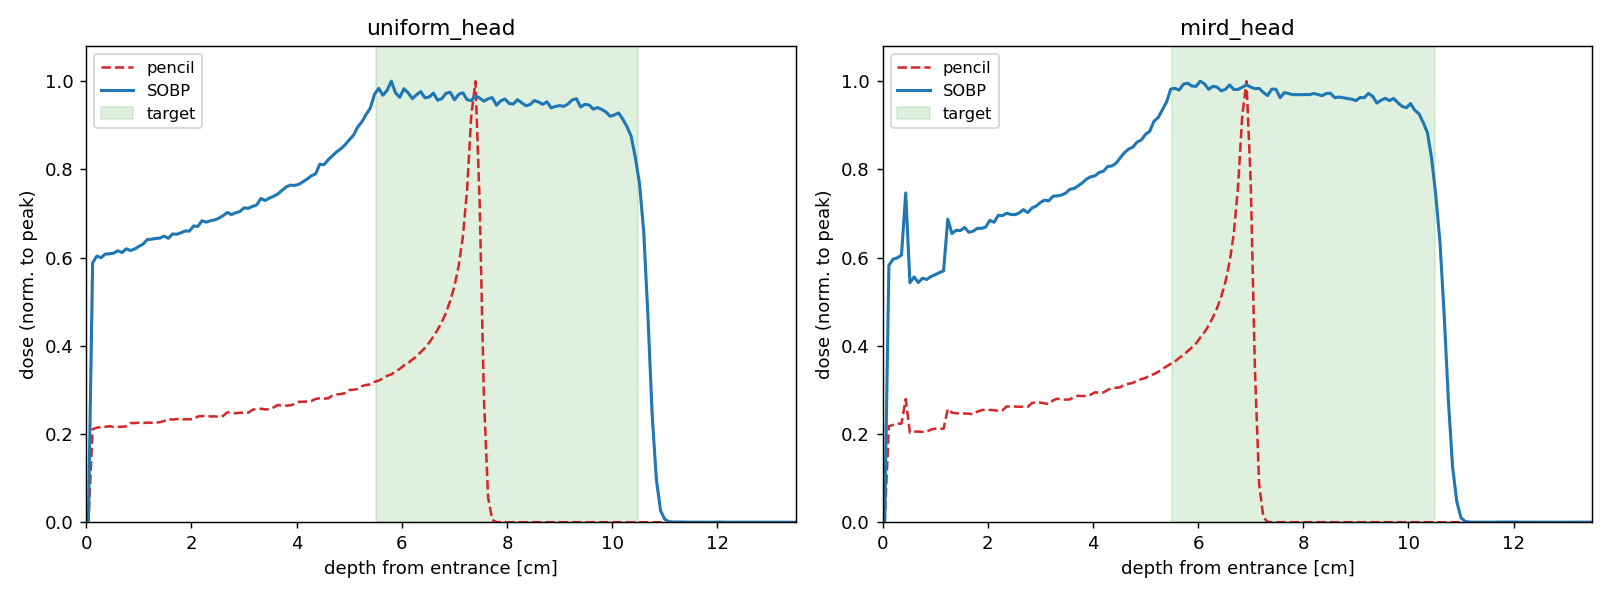
\includegraphics[width=\linewidth]{beam_compare.png}
\caption{Why a spread-out field, and what the skull does. Central-axis depth dose
(each normalised to its own peak) for a single \SI{100}{MeV} \textbf{pencil}
(dashed) and the \textbf{SOBP} (solid), in the brain-only \file{uniform\_head}
(left) and the heterogeneous \file{mird\_head} (right). The pencil deposits a
sharp peak at a single depth; the SOBP fills the whole target box (shaded). Across
the two panels, the skull's fingerprints are the small dose bumps where the beam
crosses bone (right only), and the same pencil stopping ${\sim}\SI{0.5}{cm}$
\emph{shallower} in the head with bone --- the extra stopping power the WEPL design
compensates for.}
\label{fig:compare}
\end{figure}

Running the same machinery on \file{uniform\_head} (the same envelope, brain
throughout) isolates the skull's effect. The bone demands a higher-energy field ---
WEPL window $[\SI{6.18}{},\SI{11.39}{}]\,\si{cm}$ and layers
\SIrange{88.8}{125.4}{MeV} for \file{mird\_head}, versus
$[\SI{5.69}{},\SI{10.90}{}]\,\si{cm}$ and \SIrange{84.7}{122.3}{MeV} with no bone
--- yet both land R80 on the target distal edge (\SI{10.49} vs \SI{10.52}{cm},
target \SI{10.5}{cm}) at comparable uniformity (\SI{6.2} vs \SI{8.3}{\percent}). The
skull changes the beam energy the field must deliver, not where the dose ends up:
that is what designing in WEPL buys.

\section{The handoff}
\label{sec:handoff}

The proton run gives the number of emitters \emph{produced}. A scanner measures
fewer, because it starts after the beam and acquires for a finite time. The
handoff applies the three-factor decay-kinetics expression
(\file{ptcrysp\_physics.tex}, Eq.~3) to turn the produced count $P_j$ into the
measured count $N_j$, for a chosen timing.

\paragraph{The operating point.} The standard study is in-room: a full-ring
scanner in the treatment room images the patient shortly after irradiation. The
baseline timing is $\tirr=\SI{60}{s}$, $\tdel=\SI{120}{s}$, $\tmeas=\SI{1200}{s}$.
The delay $\tdel$ is the key knob: \SI{120}{s} is about the fastest realistic
in-room delay, and longer delays are explored by varying it. A more conservative
offline point ($\tdel=\SI{300}{s}$, $\tmeas=\SI{1800}{s}$) is also provided. The
short in-room delay keeps $\Ox{15}$ abundant and dominant.

\paragraph{What the handoff writes.} The handoff writes the budget: $N_j$ per
isotope, for the chosen dose and timing, using no random numbers. A scenario may
carry several budgets that differ only in timing; the spatial source is shared. The
statistical spread of a real measurement (each count fluctuates Poisson around
$N_j$) is added later, by the downstream study.

\paragraph{Source sampling.} The detector requires $N_j$ annihilation points per
isotope. They are drawn from \file{emitters.csv} by sampling with replacement,
reproducing the spatial shape at the required count. The handoff writes only the
deterministic budget. The Poisson realisations are drawn by
\file{decay\_sampling/budget\_gen.py}, seeded as
$\text{master\_seed}+\text{realization}$ so every detector configuration sees
the identical source (a step that moves to the downstream study); the sampling
of annihilation points is done by the detector study itself.

\paragraph{Figure of merit.} The precision of the recovered proton range,
$\sigma(\text{range})$, is the error bar on a single measurement. One realisation
draws $M_j\sim\mathrm{Poisson}(N_j)$ for every isotope, forms the source, runs the
detector and the reconstruction, and fits the distal fall-off to a range estimate
$R_z$. Over $Z\sim100$ realisations,
$\sigma(\text{range})=\operatorname{std}\{R_1,\dots,R_Z\}$. The detector with the
smallest $\sigma(\text{range})$ at a fixed budget is preferred.

Each realisation resamples \file{emitters.csv} with replacement, so the
recovered range is only as well defined as the pool of \emph{distinct} emitters
near the distal edge --- the run statistics set that pool density, while the
measured counts $N_j$ are fixed by the dose and timing alone. The pool argument
and its gate, \file{analysis\_transport/distal\_pool.py}, are described in
Sec.~\ref{sec:validation}; the statistics are derived in the physics note.

\section{The scenario data product}
\label{sec:scenario}

A \emph{scenario} is the frozen output of one proton run plus its decay handoff: a
detector-independent positron-annihilation source that a downstream PET simulation
reads and turns into a measured acquisition. It is specified here as a data
product --- its files, columns and metadata, the shared coordinate frame, and the
recipe a consumer follows --- so that a scenario directory can be used from its own
contents alone. The terse machine copy ships inside every scenario as
\file{SCHEMA.md}; this section is its annotated form.

A scenario carries three logically distinct pieces of information, plus reference
and provenance files:
\begin{description}[leftmargin=1.6em]
  \item[\emph{where}] the spatial source --- the annihilation points
    (\file{emitters.csv});
  \item[\emph{how many}] the measured decays per isotope at a chosen acquisition
    timing (\file{sampling\_budget\_<scenario>.csv});
  \item[\emph{through what}] the phantom medium the \SI{511}{keV} photons traverse
    (\file{phantom\_regions.csv} $+$ \file{phantom\_material\_*}).
\end{description}
The spatial source is expensive and computed once; the number depends on dose and
timing and is a tiny separate file; the medium is implied by the run but not
carried in the point list, so it is materialised explicitly.

\subsection{Coordinate frame}
\label{sec:frame}

\begin{figure}[t]
  \centering
  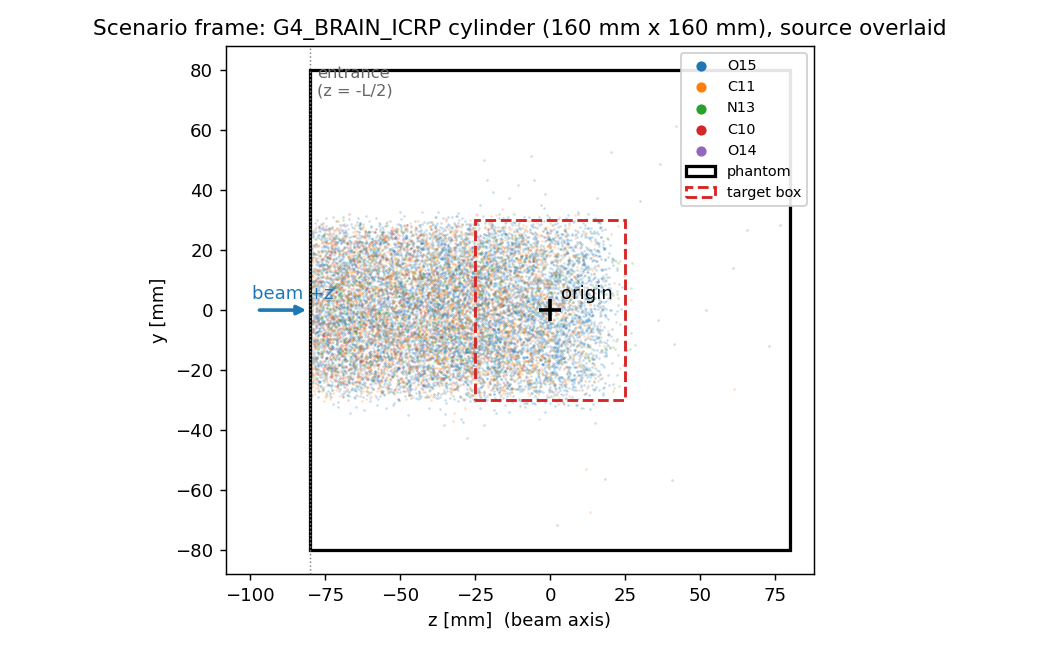
\includegraphics[width=\linewidth]{scenario_geometry.png}
  \caption{The scenario frame, drawn from \file{run\_meta.csv} with a subsample
  of \file{emitters.csv} annihilation points overlaid (one colour per isotope).
  The phantom is a cylinder centred at the origin with its axis along $+z$, the
  beam direction; the beam enters at the $z=-L/2$ face. The source cloud fills
  the proton path and tapers at the distal edge; it is laterally confined to the
  irradiated disk. The dashed box is the dose-normalisation target.}
  \label{fig:frame}
\end{figure}

All positions in a scenario --- the annihilation points, the phantom, and the
target box --- share \textbf{one Cartesian frame} (Fig.~\ref{fig:frame}). The
phantom is a cylinder centred at the origin with its axis along $+z$, the direction
the proton beam travels. It spans $z\in[-L/2,\,+L/2]$ and radius
$r=\sqrt{x^2+y^2}\in[0,R]$, with $L=\file{phantom\_length\_mm}$ and
$R=\file{phantom\_diameter\_mm}/2$. The beam enters at the $z=-L/2$ face, and depth
into the phantom from that face is
\begin{equation}
  d = z + L/2, \qquad\text{equivalently}\qquad z = d - L/2 .
  \label{eq:depth}
\end{equation}
The target-box depths in \file{run\_meta.csv} are measured from the entrance, so
they map to $z=\file{target\_*\_depth\_mm}-L/2$. A consumer that instantiates the
phantom with its centre at the origin is co-registered with the source: no offset
or rotation is needed.

\subsection{File reference}
\label{sec:files}

Units throughout: position \si{mm}, energy \si{keV} (beam energy \si{MeV}), time
\si{s} for acquisition timing, dose \si{Gy}. Each data file with run-level scalars
has a companion \file{*\_meta.csv} (a single wide row).

\paragraph{\file{emitters.csv} --- the spatial source.} One row per produced
$\bplus$ emitter; the high-statistics production shape.
\begin{center}
\begin{tabular}{@{}lll@{}}
\toprule
column & type & meaning \\
\midrule
\file{event\_id} & int & primary proton that produced it (diagnostic) \\
\file{isotope\_id} & int8 & isotope code (see \file{isotopes.csv}) \\
\file{prod\_x\_mm}, \file{prod\_y\_mm}, \file{prod\_z\_mm} & float & production point --- the truth map \\
\file{anh\_x\_mm}, \file{anh\_y\_mm}, \file{anh\_z\_mm} & float & annihilation point --- the detector source \\
\bottomrule
\end{tabular}
\end{center}
The positron range per emitter is $\file{anh}-\file{prod}$. Positrons that would
leave the phantom into air are stopped at the surface, so a small fraction
($\sim$\SI{0.6}{\percent}) have their \file{anh} pinned to the boundary. The file
holds the production \emph{shape} at the simulated statistics; the absolute
measured count is set by the budget.

\paragraph{\file{run\_meta.csv} --- run-level metadata.} One wide row: beam,
geometry, dosimetry, and provenance.
\begin{center}
\begin{tabular}{@{}lll@{}}
\toprule
column & type & meaning \\
\midrule
\file{n\_protons} & int & primaries simulated \\
\file{beam\_energy\_MeV} & float & pencil energy constant (an SOBP run's beam is its copied \file{sobp\_layers.csv}) \\
\file{beam\_sigma\_mm} & float & Gaussian beam $\sigma$ at entrance (pencil mode) \\
\file{geometry} & string & \file{cylinder} \textbar{} \file{uniform\_head} \textbar{} \file{mird\_head} \textbar{} \file{headep} \textbar{} \file{uniform\_headep} \\
\file{phantom\_material} & string & single material, or \file{multi} (per-region in \file{phantom\_regions.csv}) \\
\file{phantom\_diameter\_mm}, \file{phantom\_length\_mm} & float & phantom cylinder size \\
\file{phantom\_mass\_g} & float & phantom mass \\
\file{edep\_total\_MeV} & float & total energy deposited in the phantom \\
\file{dose\_total\_Gy} & float & whole-phantom dose for \file{n\_protons} \\
\file{target\_dose\_Gy} & float & dose in the target box for \file{n\_protons} \\
\file{target\_mass\_g} & float & target-box mass \\
\file{target\_radius\_mm} & float & target box (cylinder) radius \\
\file{target\_prox\_depth\_mm}, \file{target\_dist\_depth\_mm} & float & target faces, depth from entrance \\
\file{Np\_per\_Gy} & float & protons for \SI{1}{Gy} ($=\file{n\_protons}/\file{target\_dose\_Gy}$) \\
\file{geant4\_version}, \file{physics\_list}, \file{random\_seed} & & provenance \\
\bottomrule
\end{tabular}
\end{center}
The absolute normalisation scales production to a clinical dose $D$ via
\file{target\_dose\_Gy}: $P_j(D)=\file{count}_j\cdot D/\file{target\_dose\_Gy}$.

\paragraph{\file{depth\_dose.csv} --- the realised depth field.} One row per
\SI{1}{mm} depth bin: \file{z\_mm} (bin centre), \file{edep\_total\_MeV} and
\file{edep\_primary\_MeV} (energy deposit over the whole transverse plane, all
particles and primary protons respectively), and the on-axis core columns
\file{edep\_core\_MeV} and \file{dose\_core\_Gy} (deposit within
$r\le\SI{5}{mm}$, the latter converted to dose with the on-axis material
density). This is the run's realised Bragg/SOBP curve; the plateau metrics and
the depth-dose figures read \file{dose\_core\_Gy}.

\paragraph{\file{sampling\_budget\_<scenario>.csv} --- measured decays.} One row
per isotope: \file{isotope\_id} and \file{N\_expected}, the expected measured
decays for \SI{1}{Gy} at this timing. The companion \file{*\_meta.csv} carries
\file{scenario}, \file{source\_file}, \file{dose\_Gy}, and the acquisition timing
\file{t\_irr\_s}, \file{t\_del\_s}, \file{t\_meas\_s}. The baseline
\file{inroom} budget ($\tdel=\SI{120}{s}$) is the \file{budget.py} default;
further budgets are made by passing a label and the timing, e.g.\
\file{-{}-scenario fast -{}-t-del 60} or \file{-{}-scenario offline -{}-t-del
300 -{}-t-meas 1800}. Shorter delay keeps more short-lived $\Ox{15}$.

\paragraph{\file{phantom\_regions.csv} $+$ \file{phantom\_material\_*} --- the
medium.} The source is detector-independent but not medium-independent: a PET
simulation must propagate the \SI{511}{keV} photons through the phantom and needs
the material at each point. \file{phantom\_regions.csv} gives \emph{where} each
material is --- one row per region in the source frame, with \file{region},
\file{priority}, \file{material}, \file{solid}, semi-axes \file{a\_mm,b\_mm,c\_mm}
(cylinder: $r,r,\text{half-length}$), centre \file{cx\_mm,cy\_mm,cz\_mm}, and Euler
angles. The regions are axis-aligned; a point takes the material of the first
(lowest-\file{priority}) region containing it, else air, with ellipsoid membership
$((x-c_x)/a)^2+((y-c_y)/b)^2+((z-c_z)/c)^2\le 1$. Brain-first ordering carves the
skull shell, so no boolean solids are needed.
\file{phantom\_material\_<material>.csv} gives \emph{what} each material is: one row
per element (\file{element}, \file{Z}, \file{A\_g\_mol}, \file{mass\_fraction}),
with a companion \file{*\_meta.csv} carrying \file{density\_g\_cm3},
\file{mean\_excitation\_eV}, and $\mu/\rho$, $\mu$ and the mean free path at
\SI{511}{keV}.

\paragraph{Reference files.} \file{isotopes.csv} decodes \file{isotope\_id}
(\file{name}, \file{half\_life\_s}, \file{endpoint\_MeV}, \file{prompt\_gamma}).
\file{sobp\_layers.csv} is the beam definition. \file{SCHEMA.md} is the terse
column reference; \file{README.md} is the scenario writeup with numbers filled in;
\file{figures/} holds the run's control plots --- the phantom drawing, the
realised depth-dose, the dose--activity overlay, the validation dashboard, the
activity curves, and for SOBP runs the annotated plateau
(Sec.~\ref{sec:validation} lists which script makes which).

\subsection{How a consumer builds an acquisition}
\label{sec:use}

The scenario gives the source; the detector study realises it:
\begin{enumerate}[leftmargin=1.8em]
  \item Choose a timing budget and read $N_{\mathrm{expected},j}$ per isotope from
    \file{sampling\_budget\_<scenario>.csv}. (Rescale linearly for a dose other
    than \SI{1}{Gy}.)
  \item For each isotope $j$, draw
    $M_j\sim\mathrm{Poisson}(N_{\mathrm{expected},j})$ annihilation points by
    sampling, with replacement, the rows of \file{emitters.csv} with that
    \file{isotope\_id} (columns \file{anh\_x/y/z\_mm}). Seed reproducibly, e.g.\
    $\text{master\_seed}+\text{realization}$, so every detector configuration sees
    the identical source.
  \item From each sampled point, emit a back-to-back \SI{511}{keV} photon pair
    (isotropic direction, with the chosen non-collinearity blur).
  \item Transport the photons through the phantom defined by
    \file{phantom\_regions.csv} and \file{phantom\_material\_*}; use the same
    medium for reconstruction attenuation correction.
\end{enumerate}
All randomness (the Poisson draw, the emission directions) lives in the consumer;
the scenario itself is deterministic and seed-free, so the source is reproducible
across studies.

\subsection{Worked example: \file{cylinder\_sobp\_1e7}}
\label{sec:example}

The standard skull-base reference: a proton SOBP field delivering \SI{1}{Gy} to a
target inside a head, modelled as a homogeneous brain cylinder
(Fig.~\ref{fig:frame}).

\paragraph{Geometry and beam.} A \file{G4\_BRAIN\_ICRP} cylinder, \SI{160}{mm}
diameter $\times$ \SI{160}{mm} ($L=\SI{160}{mm}$, $R=\SI{80}{mm}$, so
$z\in[-80,80]\,$\si{mm}). The beam enters at $z=-\SI{80}{mm}$ and travels $+z$; it
is a spread-out Bragg peak painted over a uniform disk. The dose-normalisation
target box is \SI{60}{mm} diameter $\times$ \SI{50}{mm}, at \SI{55}{}--\SI{105}{mm}
depth, so by Eq.~\eqref{eq:depth} $z\in[-25,25]\,$\si{mm}. $10^{7}$ protons,
Geant4~11.4.1, \file{QGSP\_BIC\_HP}.

\paragraph{Normalisation.} The simulated target dose is
$\file{target\_dose\_Gy}\approx\num{5.97e-4}$ for $10^{7}$ protons, so reaching
\SI{1}{Gy} needs $\file{Np\_per\_Gy}\approx\num{1.68e10}$ protons; production counts
scale by that factor.

\paragraph{Source.} Per \SI{1}{Gy}, the integral yields are
$\Ox{15}\approx\num{2.5e8}$, $\Cl{11}\approx\num{1.1e8}$,
$\Nt{13}\approx\num{1.9e7}$, $\Cl{10}\approx\num{1.2e7}$,
$\Ox{14}\approx\num{8.7e6}$ (total $\approx\num{4e8}$), about $2.2\times$ the
Parodi~2008 Table~2 head values --- the expected agreement for a Geant4
cross-section model on a homogeneous brain phantom.

\paragraph{Measured decays (in-room baseline).} At $\tirr=\SI{60}{}$,
$\tdel=\SI{120}{}$, $\tmeas=\SI{1200}{s}$ the measured decays are
$N_{\Ox{15}}\approx\num{1.07e8}$, $N_{\Cl{11}}\approx\num{5.0e7}$ (total
$\approx\num{1.7e8}$), a measured $\Ox{15}/\Cl{11}\approx 2.1$. The \file{fast}
budget ($\tdel=\SI{60}{s}$) raises that ratio to $\approx 2.9$; the \file{offline}
budget ($\tdel=\SI{300}{s}$) lowers it toward the Parodi $\approx1.2$.

\paragraph{Medium.} \file{G4\_BRAIN\_ICRP}: $\rho=\SI{1.040}{g/cm^3}$, oxygen mass
fraction $0.712$, with $\mu/\rho=\SI{0.0953}{cm^2/g}$ and $\mu=\SI{0.0991}{cm^{-1}}$
at \SI{511}{keV} (mean free path \SI{10.1}{cm}) --- the attenuation a consumer
applies to the back-to-back photons and in reconstruction.

\section{Running the pipeline}
\label{sec:using}

Design the beam, run the transport, compute the budget, and freeze the result as a
scenario:
\begin{verbatim}
  python3 field_design/sobp.py --mu 0.025      # design the cylinder SOBP layers
  ./proton_transport cylinder_sobp.mac         # Geant4 run -> data/runs/<tag>/
  python3 decay_sampling/budget.py data/runs/<tag>   # -> sampling_budget_inroom.csv
  python3 tools/snapshot_scenario.py cylinder_sobp_1e7   # freeze into the scenarios repo
\end{verbatim}
For a head case the field is designed in WEPL through that phantom (from a
pencil run of its geometry), then its own macro is run:
\begin{verbatim}
  python3 field_design/sobp.py --from-run data/runs/headep_pencil_1e5
  ./proton_transport headep_sobp.mac   # also mird_head_sobp.mac, uniform_head_sobp.mac
\end{verbatim}
Full build and run instructions are in \file{CLAUDE.md}; the file columns are in
\file{common/SCHEMA.md}. A run is validated before it is frozen; the gates and
control figures are the subject of the next section.

\section{Validating a run}
\label{sec:validation}

\subsection{The run directory}
Every run owns a directory, \file{data/runs/<tag>/}, holding everything the run
produced: \file{emitters.csv}, \file{run\_meta.csv}, \file{depth\_dose.csv},
\file{phantom\_regions.csv} with the material files, the copied SOBP layer
table and its provenance meta, and \file{figures/}. The tag is derived from the
run itself --- \file{<geometry>\_<beam>\_<N>}, with the beam \file{sobp} when a
layer table is loaded and \file{pencil} otherwise, and $N$ the proton count
(e.g.\ \file{cylinder\_sobp\_1e7}) --- so the name cannot disagree with what
ran, distinct cases coexist under \file{data/runs/}, and re-running a
configuration overwrites only its own directory. In a multithreaded run the
worker threads merge into one run and the master alone writes the files.

\subsection{The gates}
Four scripts turn a finished run into a trusted one; each takes the run
directory as its argument, and the first two exit non-zero on a violation, so
they can gate a pipeline.

\paragraph{\file{check\_run.py} --- the invariants gate.} Recomputes the
geometry and normalisation invariants in plain Python from
\file{run\_meta.csv} and \file{phantom\_regions.csv}: the target-box centre
sits in a medium; the reported target mass equals $\pi r^2 L\,\rho$ for the
material at its centre (to \SI{0.5}{\percent}, tight enough to catch a
\SI{1}{\percent} density swap); the target dose is at least the whole-phantom
dose; \file{Np\_per\_Gy} is consistent with
$\file{n\_protons}/\file{target\_dose\_Gy}$; the target box fits inside the
phantom and every region inside the reported bounding box; the head regions
carve in priority order; an independent recompute of the core dose matches;
and, for an SOBP run, the field provenance (its \file{design\_geometry} and
target window match the run) and the plateau gates --- uniformity
$\le\SI{12}{\percent}$ and R80 within \SI{5}{mm} of the target distal edge.
These are the geometry bugs that carry correct units and would otherwise pass
silently.

\paragraph{\file{sobp\_metrics.py} --- plateau numbers.} Computes the plateau
dose and uniformity over the target window, R80, the proximal \SI{80}{\percent}
rise and the modulation width from \file{dose\_core\_Gy}
(Sec.~\ref{sec:field}), and draws \file{figures/sobp\_plateau.png}. With
\file{-{}-max-uniformity} and \file{-{}-r80-tol} it becomes an acceptance test.

\paragraph{\file{validate\_transport.py} --- the physics dashboard.} Renders
\file{figures/transport\_validation.png}: positron range per isotope
(endpoint-ordered), depth and radial production profiles, the production map,
emitter multiplicity, the Bragg curve split into primary and secondary deposit,
the activity--dose overlay, and the per-isotope summary table (also printed to
stdout). The sanity criteria are physical: ranges ordered by endpoint, activity
falling to zero before the Bragg peak, yields per proton at the expected
$10^{-2}$ scale.

\paragraph{\file{parodi\_cross\_check.py} --- the literature anchor.} Scales
the run's yields to \SI{1}{Gy} and compares, isotope by isotope, with Parodi
\emph{et al.}\ (2008) Table~2. Gross agreement (the expected factor
$\sim$2, Sec.~\ref{sec:example}) validates the absolute scale.

\paragraph{\file{distal\_pool.py} --- statistics for a $\sigma_R$ study.}
Counts the distinct emitters within $\pm\SI{0.5}{cm}$ of the activity distal
edge (R80 of the central-axis dose, the same depth \file{check\_run.py} gates
on) and reports the resulting pool-granularity floor on the recovered range,
of order $\text{window}/\sqrt{n}$. With \file{-{}-min-o15} it refuses a run
whose $\Ox{15}$ pool is too sparse for the planned study, before the run is
frozen.

\subsection{The control figures}
\file{make\_figures.py} reads the run's geometry and invokes the plotters that
fit the case; every figure lands in \file{<run\_dir>/figures/} and ships with
the frozen scenario.
\begin{center}
\begin{tabular}{@{}lll@{}}
\toprule
figure & script & runs \\
\midrule
\file{phantom.png} & \file{analysis\_transport/plot\_phantom.py} & all \\
\file{depth\_dose.png} & \file{analysis\_transport/plot\_depth\_dose.py} & all \\
\file{dose\_activity.png} & \file{analysis\_transport/plot\_dose\_activity.py} & all \\
\file{transport\_validation.png} & \file{analysis\_transport/validate\_transport.py} & all \\
\file{activity.png} & \file{decay\_sampling/activity\_plot.py} & all \\
\file{sobp\_g4.png} & \file{field\_design/plot\_sobp.py} & cylinder SOBP \\
\file{mird\_head.png} & \file{analysis\_transport/plot\_mird\_head.py} & head geometries \\
\file{sobp\_plateau.png} & \file{analysis\_transport/sobp\_metrics.py} & SOBP runs \\
\bottomrule
\end{tabular}
\end{center}
Two standalone plotters serve the documentation: \file{plot\_geometry.py}
draws the annotated scenario frame (Fig.~\ref{fig:frame}) and
\file{compare\_beams.py} overlays several runs' depth doses
(Fig.~\ref{fig:compare}).

\section{What to keep in mind}
\label{sec:caveats}

\begin{itemize}[nosep]
\item \textbf{The homogeneous phantoms have no internal isotope split.} A single
material gives no spatial $\Ox{15}/\Cl{11}$ variation and no biological washout;
those enter only with the layered phantom and a tissue model.
\item \textbf{Absolute yields carry a Geant4 bias.} The cross sections are
indicative rather than finely tuned; absolute counts should be read as such, while
relative comparisons between detectors are robust.
\item \textbf{The positron range sets a resolution floor}, largest for $\Ox{15}$.
\end{itemize}

\bibliographystyle{unsrt}
\bibliography{biblio}

\end{document}
